\chapter{Implementation}

% Section Introduction


\section{Type System}
The type system for the DSL is built using a subset of Scala, Python, and Cassandra's type systems. These types are shown in Figure \ref{fig:datatypes}.

\begin{figure}[h]
	\centering
	\begin{tabular}{| c | c | c | c |}
		\hline
		\textbf{Base Type} & \textbf{Python} & \textbf{Scala} & \textbf{Cassandra} \\ \hline
		Integer & int & Long & bigint \\ \hline
		Float & float & Double & double \\ \hline
		String & string & String & text \\ \hline
		Boolean & boolean & Boolean & boolean \\ \hline
		DateTime & datetime & Instant & timestamp \\ \hline
	\end{tabular}
	\caption{Primitive Types}
	\label{fig:datatypes}
\end{figure}

There were two main goals when selecting these primitive types. Firstly, every type should be able to be represented without data loss in all parts of the system. Secondly, it should be possible to represent the types in protobuf format, as this would allow for easy serialisation of result data. All types except DateTime are can be converted to protobuf natively, and DateTimes are supported by serialising as an ISO8601 formatted string \cite{iso_8601}.

Designing the actual interfaces to represent these values presents a challenge. To be able to read and manipulate these types in Scala at runtime, the raw primitive types cannot be used. This is because the only common supertype of all primitive types is \textit{Any}, as shown in Figure \ref{fig:scala-unified-types}. There is effectively no information shared between all supported types in the system. To discover which type a given value is (or if the type is even supported), the system would have to perform runtime type checks against all possible supported types. These checks would add a significant amount of overhead, and as a result this approach was not selected.

\begin{figure}[h]
	\centering
	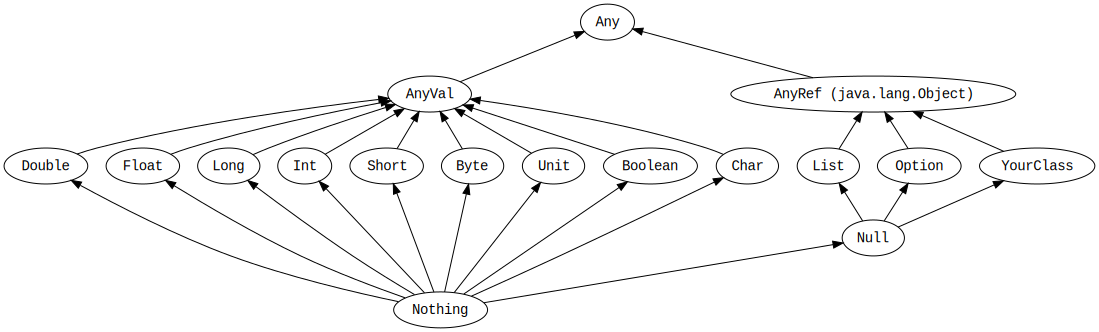
\includegraphics[width=0.8\textwidth]{chapters/diagrams/implementation/unified-types-diagram}
	\caption{Scala Unified Types \protect\cite{scala_unified_types}}
	\label{fig:scala-unified-types}
\end{figure}

Another possible approach to solving this problem is to create a lightweight container class, which holds the value, and the type information about the value at runtime. This means that the system only needs to perform the runtime type check once in order to create the correct class instance. Due to limitations of Java, this conceptual solution is not entirely straightforward to implement. The container class would use a generic type parameter which stores the type information of the value inside the container. A given row of data would need to support multiple types of data stored together, and this is not possible using generics as the type information of the generic is erased at runtime \todo{reference}. 

The container class could instead be defined as an interface, and each supported type provides an implementation of that interface, but this is not much better than the primitive type solution, as the runtime type check simply becomes a runtime pattern match on the class instance. A solution that exploits some kind of polymorphism is preferred.

Scala provides an feature known as ClassTags \todo{reference}. These allow the erased type information to be recorded, and also allow equality checks to be performed between ClassTags. By storing a ClassTag instance, we can implement type equality checks between values in the system, to determine if they are of the same type. Furthermore, we can use this type information later to determine what types are accepted and returned by FieldExpressions.

This is defined in the system using a base interface \textit{ValueType}, which captures the ClassTag requirement. This interface is used as part of both \textit{TableField}, which captures field information (name and type), and \textit{TableValue}, which captures value information (value and type). Implementations for all the supported types are then provided for both \textit{TableField} and \textit{TableValue}. \todo{insert figure ref} shows the hierarchy of these types. 

\missingfigure{ValueType - TableField - TableValue hierarchy} 

\subsection{Result Model}
This hierarchy of classes provides everything needed to define computation results in the system. Headers are defined as a sequence of TableFields, and results are defined as a two-dimensional array of \texttt{Option[TableValue]}. As defined in the requirements, null values must be supported, but the use of nulls in Scala is discouraged. Instead, Option is preferred as it is supported by all the typical functional methods. In this model, values are represented by \texttt{Some(TableValue())}, and null values are represented by \texttt{Nothing}. \todo{insert figure ref} shows what an example result looks like using this definition.

\missingfigure{Visual of TableResult}

\section{Domain Specific Language}
The user's interaction with the framework is driven entirely by the Domain Specific Language (DSL). The language allows the user to define expressions, comparisons, aggregates, and then use these to define computations like Select, Filter and Group By. As per the requirements, the DSL has been modelled with SQL-like syntax.

\subsection{FieldExpressions}
FieldExpressions are the key building block of the DSL. They allow the user to define arbitrary row-level calculations to be used as part of more complex operations. FieldExpressions are defined as an interface, which provides a standard set of methods, and there are three subclasses that provide implementations:

\begin{itemize}
	\item Values: define literal values which never change across all rows
	\item Fields: when iterating over the rows of a result, gets the value from the named field in the current row.
	\item FunctionCalls: perform arbitrary function calls using further FieldExpressions as arguments.
\end{itemize}

Examples of FieldExpressions are shown in Figure \ref{fig:field-expressions-examples}.

\begin{figure}[h]
	\centering
	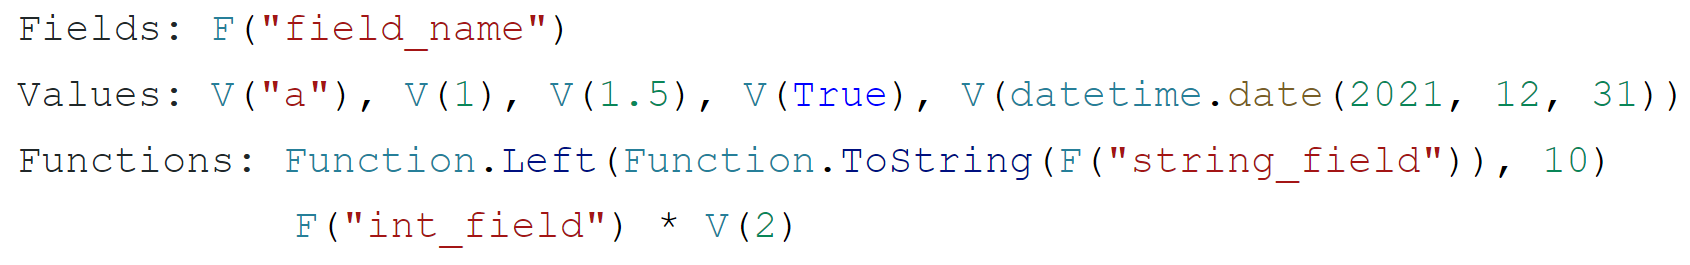
\includegraphics[width=0.8\textwidth]{chapters/diagrams/implementation/field-expressions-examples}
	\caption{Examples of FieldExpressions}
	\label{fig:field-expressions-examples}
\end{figure}

Many basic functions have been implemented, including arithmetic, string and cast operations. However, the function system is designed to be extensible. A number of helper classes are defined to allow the creation of basic unary, binary and ternary functions, but FunctionCall is itself an interface which can be given completely custom implementations if required. The main constraints on the functions that can be defined are that only the 5 primitive input types are supported.

\paragraph{Type Resolution} 
Type Resolution on FieldExpressions is performed in two stages: a resolution step, and an evaluation step. The resolution step takes in type information from the header of the input result, and verifies that the FieldExpression is well typed with regards to that result. This is necessary for Fields, which may be valid for one result but invalid for another, for example if the field name is missing from the result. The evaluation step performs the computation on a row from that result without any type checking. 

This two-step process has a number of benefits. The resolution step enables a form of polymorphism on some functions like arithmetic operations. At the resolution step, these functions determine what types are returned by their sub-expressions, and resolve to the correct version for evaluation. For example, the add function can resolve to AddInt, AddDouble, or Concat for strings. Also, there is reduced overhead at runtime as type checking does not need to be performed for each row - unchecked casts are used here instead.

\paragraph{Named Expressions}
When performing a Select operation, the output fields are all expected to be named. This allows the user to repeatedly chain operations by referencing fields from the input. Therefore, FieldExpressions have a method to allow them to be named. When this method is called, the FieldExpression is wrapped as a tuple with the name into a NamedFieldExpression. Field references are able to reuse their previous name automatically to reduce the need for repeated naming calls. 

% Abstract class implementation
% - isWellTyped
% - doesReturnType
% - resolve/evaluate steps
% - named/unnamed

\subsection{FieldComparisons}
FieldComparisons are another key building block of the DSL. They allow the user to define arbitrary row-level comparisons. FieldComparisons use a two-step resolution-evaluation process. This is in place to accommodate the two-step process that already exists for FieldExpressions. They are defined as an interface, and there are four subclasses that provide implementations:

\begin{itemize}
	\item Null Checks: takes a single FieldExpression as input, and filters out rows where it is null/not null.
	\item Equality Checks: performs an equal/not equal check on two FieldExpressions.
	\item Ordering Checks: applies an ordering comparator to two FieldExpressions.
	\begin{itemize}
		\item Supports $<$, $<=$, $>$, $>=$.
	\end{itemize}
	\item String Checks: applies a string comparator to two FieldExpressions
	\begin{itemize}
		\item Supports contains, starts with and ends with (both case sensitive and insensitive versions).
	\end{itemize}
\end{itemize}

Examples of FieldComparisons are shown in Figure \ref{fig:field-comparisons-examples}.

\begin{figure}[h]
	\centering
	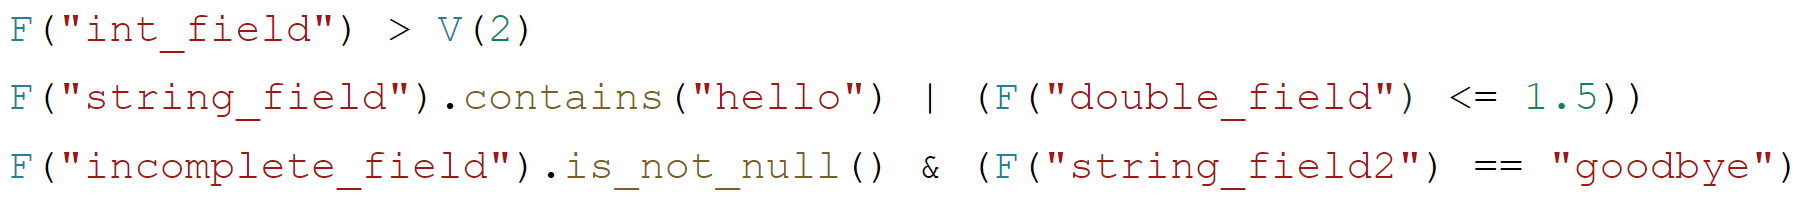
\includegraphics[width=0.8\textwidth]{chapters/diagrams/implementation/field-comparisons-examples}
	\caption{Examples of FieldComparisons}
	\label{fig:field-comparisons-examples}
\end{figure}

\paragraph{Combined Comparisons}
The user is able to combine multiple FieldComparisons using AND/OR operators. This is a lightweight wrapper around Scala's own AND (\texttt{\&\&}) and OR (\texttt{||}) boolean operators, meaning optimisations like short circuiting operate as normal with no extra work.

\subsection{Aggregate Expressions}
Aggregate Expressions are the final part of the DSL. These are used only as part of Group Bys, and allow the user to define methods of aggregating all rows of a result. Aggregate Expressions take a NamedFieldExpression as an argument, and compute a single row output from any number of input result rows.

The system supports Min, Max, Sum, Average, Count, and String Concatenation operations. These aggregates are polymorphic where possible. For example, minimum and maximum handle numeric types numerically and strings lexicographically.

\todo{expand + examples}

\subsection{Table Commands}
Given the above building blocks of the DSL, table operations are defined to perform transformations over any number of rows on a table. The system supports Select, Filter and Group By transformations. The user is able to define these sequentially to produce a full query. The result of the previous transformation is passed as the input to the next transformation.

\todo{example figure to show sequential table transformations}

\paragraph{Select}
The Select operation takes any number of NamedFieldExpressions.

\paragraph{Filter}
The Filter operation takes a single FieldComparison, or a number of FieldComparisons combined using boolean operators.

\paragraph{Group By}
The Group By operation takes any number of NamedFieldExpressions to act as unique keys, as well as any number of aggregate expressions which will be computed for each combination of unique keys.

\subsection{Protocol Buffer Serialisation}
All components of the DSL have been designed to be serialised to protobuf format. This allows any queries written by the user to be passed around the system using gRPC, and if required the query can also be serialised to a file. The results of a query are also serialisable, to allow the system to return query results to the user. gRPC has a size limit of 4MB for individual messages, so results are split up by row and streamed individually.

\subsection{Python Implementation}
The Python frontend is designed to be straightforward to use, hiding the complexities of the computation being performed in the backend. A number of Python-specific features were used to help with this.

Python allows developers to override common operators, including arithmetic ($+$, $-$, $*$, $/$) and comparison ($<$, $>$) with custom definitions. These are known as double underscore \textit{(dunder)} methods. The Python implementation of FieldExpression overrides the arithmetic operators, as well as comparison operators to allow the user to automatically generate function calls and FieldComparisons, without having to write the full, verbose definition.

Furthermore, query results can be converted from their protobuf definition as received from the server to a pandas DataFrame \cite{reback2020pandas}. This decision was made because pandas is one of the most commonly used frameworks for data analysis in Python. In the 2022 Stack Overflow Developer Survey, it was the third most popular non-web framework \cite{stackoverflowsurvey2022}. Therefore, it is likely that the intended users of the system will have prior experience performing data processing using DataFrames.

\section{Initial Attempts}
% stateless select/filter computations - use cassandra and table explanation from earlier

\subsection{Cassandra}
% Partitioning implementation

\section{Cassandra Data Co-Location}
% Workers detect closest cassandra nodes
% Cassandra provides information about which nodes hold which data
% Orchestrator uses this to provide optimal worker assignments for partitions

\section{Tables}
% Row-level operations only
% Select / Filter implementation
	
\section{Query Plan}
% Overview of final model
% Data Sources - Anywhere where new partitioning is required
% Tables - row level operations
% Full/partial query plan - components
% Source data fetching

\section{Group By}
% Hashing
% shuffling
% computation

\section{Worker}
% Overview of worker functionality

\subsection{Table Store}
% table cache - actor system, store model

\subsection{Spill to Memory}
% spill to memory - least recently used

\section{Orchestrator}
% Collating results from workers - akka actors

\section{Kubernetes}
% how it all fits together
% K8s setup
\subsection{K8ssandra}
% K8ssandra nodes

\subsection{Worker Scheduling}
% Worker scheduling rules - affinity to K8ssandra, anti-affinity to other workers


